\documentclass[12pt,a4paper]{article}
\usepackage[margin=22mm]{geometry}
\usepackage{amsmath,amssymb}
\usepackage{booktabs}
\usepackage{enumitem}
\usepackage[most]{tcolorbox}
\usepackage{tikz}
\usepackage{fancyhdr}
\usepackage{lastpage}
\usepackage{hyperref}
\definecolor{worksheetblue}{HTML}{145DA0}
\definecolor{answergold}{HTML}{FFF4CC}
\pagestyle{fancy}
\fancyhf{}
\lhead{Mathematics workshop}
\rhead{Practice sheet 04}
\cfoot{Page \thepage\ of \pageref{LastPage}}
\newtcolorbox{taskbox}[1]{colback=blue!3,colframe=worksheetblue,fonttitle=\bfseries,title=#1}
\newtcolorbox{hintbox}[1]{colback=answergold,colframe=orange!60!black,fonttitle=\bfseries,title=#1}

\begin{document}
\begin{center}
  {\Large\sffamily\bfseries Linear models and scale}\\[4pt]
  {\large Practice sheet 04}\\[6pt]
  Name: \rule{0.34\linewidth}{0.4pt}\hfill Date: \rule{0.20\linewidth}{0.4pt}
\end{center}

\begin{taskbox}{How to use this sheet}
Show the reasoning that leads to each answer.  Use the hint boxes as a model
for a worked solution, or hide them when printing a student-only copy.
\end{taskbox}

\section*{Problems}
\begin{taskbox}{Problem 1 — proportional change}
A sensor reports 18 units after 6 minutes and 42 units after 14 minutes.
Assuming a linear trend, find the rate of change and predict the reading at
20 minutes.
\end{taskbox}
\begin{hintbox}{Worked solution}
The slope is
\[
  m=\frac{42-18}{14-6}=3.
\]
Using the first observation, the intercept is $18-3(6)=0$, so the model is
$y=3t$.  At 20 minutes the predicted reading is $60$ units.
\end{hintbox}

\begin{taskbox}{Problem 2 — compare two plans}
Plan A costs a fixed 24 credits plus 5 credits per sample.  Plan B costs 9
credits plus 8 credits per sample.  For how many samples do the plans cost the
same, and which plan is cheaper for 12 samples?
\end{taskbox}
\begin{hintbox}{Worked solution}
Set the costs equal: $24+5n=9+8n$, giving $n=5$.  At 12 samples, Plan A costs
84 credits and Plan B costs 105 credits, so Plan A is cheaper.
\end{hintbox}

\begin{taskbox}{Problem 3 — explain the model}
Write one sentence describing a limitation of extrapolating a linear model far
outside the range of observations.
\end{taskbox}
\begin{hintbox}{Example response}
The relationship may change beyond the measured range, so a linear trend can
produce physically impossible or poorly calibrated predictions.
\end{hintbox}

\section*{Extension}
Use the axes below to sketch $y=3t$ and mark the two observations from Problem
1.  Add a short note describing what evidence would make the linear assumption
more credible.
\begin{center}
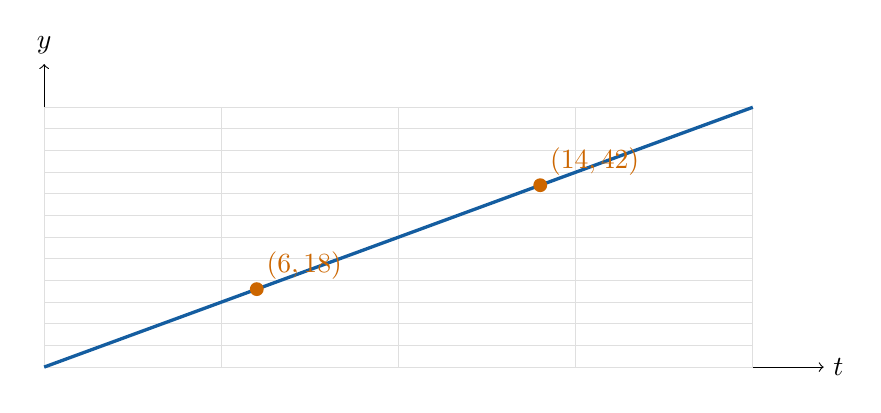
\begin{tikzpicture}[x=0.45cm,y=0.055cm]
  \draw[->] (0,0) -- (22,0) node[right] {$t$};
  \draw[->] (0,0) -- (0,70) node[above] {$y$};
  \draw[step=5,gray!25] (0,0) grid (20,60);
  \draw[very thick,worksheetblue] (0,0) -- (20,60);
  \fill[orange!80!black] (6,18) circle (2.5pt) node[above right] {$(6,18)$};
  \fill[orange!80!black] (14,42) circle (2.5pt) node[above right] {$(14,42)$};
\end{tikzpicture}
\end{center}

\vfill
\begin{center}\small\textit{Replace the fictional values with your own class data and add or remove task boxes as needed.}\end{center}
\end{document}
